\documentclass{article}
\title{Introduction to Wireless Networks Midterm Review}
\usepackage{graphicx}
\begin{document}

\section{Introduction}
Wireless networks can be classified according to several characteristics:
\begin{enumerate}
		\item{\textbf{Infrastructure}}
		\item{\textbf{mobility}}
		\item{\textbf{size}}
\end{enumerate}

Next, we have to define what a \textbf{ad-hoc network} is. An ad-hoc network is a neetwork which does
not rely on routers or traditional type of infrastructure, but has several \textit{nodes} which can
communicate with other nodes in that particular network.

Ad hoc netorks can be seen in several different places, such as devices that need to communicate with other devices but
don't necessarily share that info with any other outside source. These include: vehicles, communities, satellites, and sensors. 

\textbf{Based on infrastructure}

These types of networks are usually used in remote areas, to bring mobile IP to rural areas or establish communications.
They are mostly ad-hoc networks, and act as one-hop access points. They have multi hop wireless access links in common.

\textbf{Based on Mobility}

In such scenarios, why would wireless networks be necessary? Clearly the terrain is a big obstacle. They might require
lower maintenance, since once they are installed they might require less to keep them operational (cost-effectiveness). 
Such networks are called \textbf{\textit{static wireless networks}}.

Another type of wireless network based on mobility might be \textbf{\textit{mobile wireless networks}}. These networks
might require some of the elements in the network to be moving. In these cases, some of the challenges involve keeping
open connections when moving, and particularly when switching to other networks. How do we keep the channel open?

\textbf{Based on Size}

Different types of wireless networks involve keeping connections over shorter or longer distances. There are: body networks,
which might operate within a single human/animal body (like a pacemaker?); personal area networks, which might involve a bigger
space such as a home; local area networks, like in restaurants and office spaces; metropolitan networks, which might give 
coverage to an entire city; and wide area networks (wide bois), which might be used for cellular and satellite networks.

There are many different examples where one of these networks might be used in the real world, obviously. The healthcare 
industry would need different devices to be communicating to monitor a patient's health. Mesh networks might be able to 
provide internet access to different remote areas. Autonomous vehicles would clearly need to be relaying their current
position to other vehicles on the road, in order to experience tranquility. And finally sensor networks could be utilized
for monitoring habitats or severe weather conditions.

\hspace{10mm}\textbf{\textit{Example: autonomous vehicles}}

The increased popularity of autonomous vehicles make them a prime example of reliance on mobile ad-hoc networks.
Driving and parking would need to communicate curent conditions to other automobiles to ensure a customer's 
safety and convenience are guaranteed with the highest guarantee of confidence.

Other uses of mobile ad-hoc networks might involve multiplayer games.

Continuing the analogy of vehicles, there would also have to be a way to communicate information between the road and 
the vehicle. When a vehicle is travelling at a high speed, it would spend less time connected to a single access point.
Thus making the necessary verification and handshaking messages in this short amount of time would need to be done even 
fastetr. Luckily the results show that this is plenty of time for these interacitons to take place.

\hspace {10mm}\textbf{Community Wireless Newtworks}

With these types of networks, we could potentially create a network that provides connectivity to an entire metro area, 
such as iTaiwan and TPE-Free, etc... These networks are designed to ve static, since the access points are installed 
and then set there for the users to access depending on their location. Also, there are mesh networks present since they 
aim to connect to s many nodes as possible.

These networks have particular use in these situations. They reduce the physical infrastructure cost, allow for unplanned 
expansion, and can extend coverage to areas which previously did not have internet. That's why they enjoy ample usage in 
developing nations.

However, it is not clear whether the 802.11 protocol is suited for these types of netowrks, since it might not be the best option
over distances this long. Also, using TDMA (time division multiple access might take away some of those issues).

\hspace {10mm}\textbf{Sensor Networks}

With these cheap sensors, we are able to monitor entire populations, such as zebras with attached collars. Some of the 
zebras in the population were given collars and monitored. This example brought extra difficulties in that there were 
no real fixed nodes, since all the zebras were moving. There was no infrastructure, large distances, and low power nodes.
\newpage
\section{Transmission Fundamentals}

There are some criteria when talking about transmission media:
\begin{enumerate}
	\item{\textbf{Transmission Media}}: physical path between transmitter and receiver

	\item{\textbf{Guided Media}}:when waves are guided along a solid medium.

	\item{\textbf{Unguided Media}}:Only provide means of delivering signals but does not guide EM transmission.
\end{enumerate}

Since we are dealing with physical waves, we can choose from different places of the EM spectrum. All the way from low-frequency
radio waves to IR waves, depending on the distance we might need ot transmit.

\hspace{10mm}\textbf{Broadcast Radio}

For bradcast radio, the waves are transmitted in an omnidirectional manner from the source, which gives the antennas more 
freedom in choosing an alignment convenient to them.

\hspace{10mm}\textbf{EM signal}

An electromagnetic wave is a function of either time or frequency (maybe both?).

\hspace{10mm}\textbf{Time Domain}

An analog signal might be considered a continuous function. The signal varies in value at a given time, but is transmitted in
an uninterrupted fashion. There might be some variation in the intensity of the signal.

In contrast, digital signals only vary between to fixed states, from one constant state to another.

A periodic signal is one that can repeat over time.

An aperiiodic signal does not repeat over time. The amplitude is the maximum value or strength of a frequency over time and is 
usually measured in volts.

The period(T) is the amount of time it takes for one repetition of the signal and is defined by $$T = 1/f$$  
The phase ($\phi$)  is the measure of the relative position of the wave. The wavelength ($\lambda$) is the amount
of space s physical signal occupies(distance between correpsonding points of corresponding cycles).

The equation for a general sine wave is $$s(t)= Asin(2\pi ft + \phi)$$.
By modifying these variables, we can move the function around in all sorts of funny ways.

\hspace{10mm}\textbf{Frequency Domains}
There are some important concepts in the frequency domain of waves. The \textit{fundamental frequency} is the frequency when all
components of a signal are integer multiples of another.

The \textit{spectrum} is a range of frequencies that the signal contains.

The \textit{absolute bandwidth} of a signal is the width of the spectrum of the signal.

Any analog signal can be shown to be a combination of sine waves with different values. The period of the total signal is 
equal to the period of the fundamental frequency.

\hspace{10mm}\textbf{Relationship Between Data Rate and Bandwidth}

The greater the bandwidth, the greater the capactity of information that can be carried; however, the cost of transmission is 
also greater.

Digital waveforms can have infinite bandwidth, but the transmission system will limit what bandwidths are acceptable. 
However, this limitation can create distortions.

\hspace{10mm}\textbf{Data Communications Terms}
\begin{enumerate}
		\item{\textbf{Data}}: entities that convey meaning or information.
		\item{\textbf{Signal}}: electric or EM representations of the data.
		\item{\textbf{Transmission}}: Communication of data by the propagation and processing of signals.
\end{enumerate}

There are both \textit{analog} and \textit{digital} signals. They can be used for different things. For example, analog signals might
be used for audio and video, while digital signals are used for text.

\hspace{10mm}\textbf{Analog}

As mentioned, analog is a varying wave that can be transmitted with a varying frequency. Analog signals can carry both analog and
digital data, because the digital signal can be converted to analog and vice versa.

\hspace{10mm}\textbf{Digital}

Digital signals consist only of voltage pulses, which can vary from 1 to 0. Tranmsitted through copper wires and can be cheaper 
to send than their analog counterparts. They usually don't suffer from noise interference, but they can suffer from attentuation,
or weakening of the signal with more distance covered. Can also carry both analog and digital data.

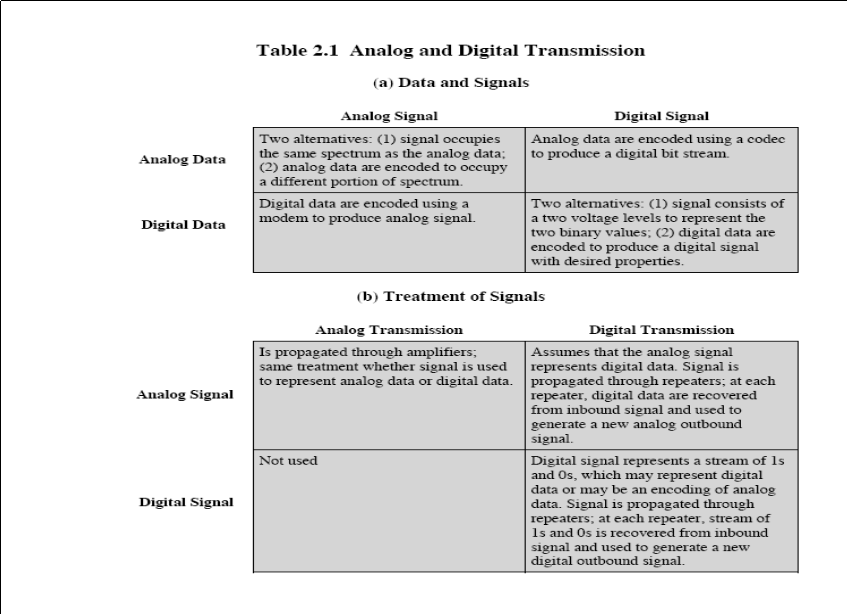
\includegraphics[scale=.25]{signals}

Why would we choose these specific methods for transmission?
\begin{enumerate}
		\item{\textbf{Digital Data, Digital Signal}}: the equipment for encoding is less expensive then D2A equipment.
		\item{\textbf{Analog Data, Digital Signal}}: conversion permits use of modern digital transmission and switching equipment.
		\item{\textbf{Digital Data, AnalogSignal}}: Depending on the media, it might only propagate analog signals, like optical 
			fibre and satellite.
		\item{\textbf{Analog Data, AnalogSignal}}: Data is easily converted between analog data and transmission.
\end{enumerate}
When we tranmsit analog signals, we don't regard the content. Because the signal suffers from attenuation, we can amplify the 
signal periodically, however these amplifiers might cause distortion. These errors are acceptable in analog data, but can cause
errors in digital transmissions

On the other hand, digital transmission is concerned with the content of the signal. Attenuation can cause the data to become 
corrupted. Digital repeaters  can achieve greater distance than amplifiers, and recover the original signal. can achieve greater distance than amplifiers, and recover the original signal.

	\textbf{Channel Capacity}: Maximum amount of data that can be transmitted through a channel. 

The signal to noise ratio can be described by the formula
				$$(SNR)_dB = 10\log_{10} \frac{signal power}{noise power} $$
A high SNR indicates that the signal is strong and will require fewer intermediate repeaters on its propagation.

The Shannon Capacity Formula is determined by
				$$C = B\log{2}(1+SNR)$$
However, th is is just a theoretical maximum. Usually much lower rates are achieved.

\newpage
\section{Antennas and Propagation}

An antenna is an electrical conductor or system of conductors.
\begin{enumerate}
		\item{\textbf{Transmission}}: radiates EM energy into space.
		\item{\textbf{Reception}}: collects EM energy from space.
\end{enumerate}

Sometimes the same antenna can be used for transmission and reception.

\hspace{10mm}\textbf{Radiation Patterns}

\textbf{Radiation Pattern}: graphical representation of an antenna's radiation properties, usually shown as two dimensional cross
section.

\textbf{Beam Width}: The mmeasure of the directivity of an antenna.

\textbf{Reception Pattern}: receiving antenna's equivalent of radiation patterns.

There are different types of antennas:
\begin{enumerate}
		\item{\textbf{Isotropic Antenna}}: This type of antenna usually radiates power equally in all directions,
				can be idealized.

		\item{\textbf{Dipole Antenna}}: can either be half-wave (Hertz) or quarter-wave (Marconi)

		\item{\textbf{Parabolic Reflective Anrtenna}}

\end{enumerate}
\hspace{10mm}\textbf{Antenna Gain}

\textbf{antenna gain}:the power output in a particular direction compared to that produced by a perfect omnidirectional antenna.

\textbf{Effective Area}: Related to physical size and the size of the antenna.

The relationship between antenna gain and effective area is:
$$G=frac{4\pi A_e}{\lambda ^2} = frac{4\pi f^2 A_e}{c^2}$$

Where G is the antenna gain, $A_e$ is the effective area, f is the carrier frequency, c is the speed of light, $\lambda$ is the carrie 
frequency.

There also are different ways of propagating EM waves, such as ground-wave, sky-wave, and Line-of-Sight propagation.
\begin{enumerate}
		\item{\textbf{Ground-wave propagation}}: Follows the contour of the Earth, can go consiserable distances with freq up to 
				2MHz. Used by AM radio for example.
		\item{\textbf{Sky-Wave propagation}}: The wave is reflected from the ionosphere back to Earth and travels in a zig-zag to
				receiver. Waves are refracted from the ionosphere. Used by amateur radio.
		\item{\textbf{Line-of-Sight propagation}}: The sender and receiver must be within line of sight to each other. In
				a sattelite communication, any signal above 30MHz is not reflected. On the ground the antennas have to be
				within effective line of sight to be able to communicate.
\end{enumerate}
				Optical line of sight is given by the formula $d = 3.57\sqrt((K)h)$
Where d is the distance , h is the height, and K is the adjustment factor for refraction (rule of thumb is 4/3).

There are also several factors which can impair wireless transmission.

\hspace{10mm}\textbf{Attenuation}

The strength of a signal can weaken with distance through a medium. The signal's strength must be enough at least so 
that the receiver's circuitry can interpret the signal. The level must also be higher than the noise to avoid possible
errors. 

The greater the frequency, the greater the distortion.

\hspace{10mm}\textbf{Free Space Loss}

Free space losss is given by the formula $$\frac{P_t}{P_r} = \frac{(4\pi d)^2}{\lambda ^2}$$

Where P is the power at the sending and receiving antenna, $\lambda$ is the carrier wavelength , d is the distance, c is the speed of
light.

\hspace{10mm}\textbf{Thermal Noise}

Thermal noise is due to the agitation of electrons. Unfortunately, it is present in all electronic media and cannot be eliminated.

Can be affected by temperature. 

Particularly affects satellites.

\textbf{Intermodulation Noise}: Occurs when two signals with different frequencies share the same medium.

\textbf{Crosstalk}: unwanted coupling between signal paths.

\textbf{Impulse Noise}: irregular noise spikes or pulses. These have a short duration and a high amplitude (like screeches almost). 
Can be caused by EM disturbance. 

Other imapairments include atmospheric conditions like water vapor and oxygen. Also, signals can be reflected or refracted depending 
on the objects in the way.

\hspace{10mm}\textbf{Multipath Propagation}

Signal can either be reflected, refracted, or diffracted. \textit{reflection} involves a wave hitting a larger surface. 

\textit{diffraction} is the same but with a body that is inpenetrable. 

\textit{scattering} occurs when the wave hits an object roughly of the same size.

All of these factors can cause different signals to arrive at different rates. If these rates undergo destructive interference, 
detection might be more difficult. 


\hspace{10mm}\textbf{Error correction Mechanisms}

Due to the inherently unstable nature of wireless transmission, we need a way to detect if information has been corrupted during
transmission. The receiver does the following operations. The error corecting function is performed on the incoming bits, and 
if they don't match, then we know there has been at least one error. 



\end{document}
